\documentclass[12pt,letterpaper]{article}\usepackage[]{graphicx}\usepackage[]{color}
%% maxwidth is the original width if it is less than linewidth
%% otherwise use linewidth (to make sure the graphics do not exceed the margin)
\makeatletter
\def\maxwidth{ %
  \ifdim\Gin@nat@width>\linewidth
    \linewidth
  \else
    \Gin@nat@width
  \fi
}
\makeatother

\definecolor{fgcolor}{rgb}{0.345, 0.345, 0.345}
\newcommand{\hlnum}[1]{\textcolor[rgb]{0.686,0.059,0.569}{#1}}%
\newcommand{\hlstr}[1]{\textcolor[rgb]{0.192,0.494,0.8}{#1}}%
\newcommand{\hlcom}[1]{\textcolor[rgb]{0.678,0.584,0.686}{\textit{#1}}}%
\newcommand{\hlopt}[1]{\textcolor[rgb]{0,0,0}{#1}}%
\newcommand{\hlstd}[1]{\textcolor[rgb]{0.345,0.345,0.345}{#1}}%
\newcommand{\hlkwa}[1]{\textcolor[rgb]{0.161,0.373,0.58}{\textbf{#1}}}%
\newcommand{\hlkwb}[1]{\textcolor[rgb]{0.69,0.353,0.396}{#1}}%
\newcommand{\hlkwc}[1]{\textcolor[rgb]{0.333,0.667,0.333}{#1}}%
\newcommand{\hlkwd}[1]{\textcolor[rgb]{0.737,0.353,0.396}{\textbf{#1}}}%

\usepackage{framed}
\makeatletter
\newenvironment{kframe}{%
 \def\at@end@of@kframe{}%
 \ifinner\ifhmode%
  \def\at@end@of@kframe{\end{minipage}}%
  \begin{minipage}{\columnwidth}%
 \fi\fi%
 \def\FrameCommand##1{\hskip\@totalleftmargin \hskip-\fboxsep
 \colorbox{shadecolor}{##1}\hskip-\fboxsep
     % There is no \\@totalrightmargin, so:
     \hskip-\linewidth \hskip-\@totalleftmargin \hskip\columnwidth}%
 \MakeFramed {\advance\hsize-\width
   \@totalleftmargin\z@ \linewidth\hsize
   \@setminipage}}%
 {\par\unskip\endMakeFramed%
 \at@end@of@kframe}
\makeatother

\definecolor{shadecolor}{rgb}{.97, .97, .97}
\definecolor{messagecolor}{rgb}{0, 0, 0}
\definecolor{warningcolor}{rgb}{1, 0, 1}
\definecolor{errorcolor}{rgb}{1, 0, 0}
\newenvironment{knitrout}{}{} % an empty environment to be redefined in TeX

\usepackage{alltt}
 \usepackage[left=2cm,right=2cm,top=2cm,bottom=2cm]{geometry}
\usepackage[ansinew]{inputenc}
\usepackage[spanish]{babel}
\usepackage{amsmath}
\usepackage{amsfonts}
\usepackage{amssymb}
\usepackage{dsfont}
\usepackage{multicol} 
\usepackage{subfigure}
\usepackage{graphicx}
\usepackage{float} 
\usepackage{verbatim} 
\usepackage[left=2cm,right=2cm,top=2cm,bottom=2cm]{geometry}
\usepackage{fancyhdr}
\pagestyle{fancy} 
\fancyhead[LO]{\leftmark}
\usepackage{caption}
\newtheorem{definicion}{Definci\'on}
\IfFileExists{upquote.sty}{\usepackage{upquote}}{}
\begin{document}

\begin{titlepage}
\setlength{\unitlength}{1 cm} %Especificar unidad de trabajo


\begin{center}
\textbf{{\large UNIVERSIDAD DE EL SALVADOR}\\
{\large FACULTAD MULTIDISCIPLINARIA DE OCCIDENTE}\\
{\large DEPARTAMENTO DE MATEM\'ATICA}}\\[0.50 cm]

\begin{picture}(18,4)
 \put(7,0){
\includegraphics[width=4cm]{minerva.jpg}}
\end{picture}
\\[0.25 cm]

\textbf{{\large Licenciatura en Estad\'istica}\\[1.25cm]
{\large Control Estadistico del Paquete R }\\[2 cm]
%\setlength{\unitlength}{1 cm}
{\large  \textbf{''UNIDAD DOS"}}\\
{\large  \textbf{Pr\'actica 10 - An\'alisis de una variable bidimensional (categ\'orica, continua) }}\\[3 cm]
{\large Alumna:}\\
{\large Martha Yoana Medina S\'anchez}\\[2cm]
{\large Fecha de elaboraci\'on}\\
Santa Ana - \today }
\end{center}
\end{titlepage}

\newtheorem{teorema}{Teorema}
\newtheorem{prop}{Proposici\'on}[section]

\lhead{UNIDAD DOS}
\chead{PR\'ACTICA 10}
\lfoot{LICENCIATURA EN ESTAD\'ISTICA}
\cfoot{UESOCC}
\rfoot{\thepage}
%\pagestyle{fancy} 

\setcounter{page}{1}
\newpage

\begin{center}
\subsubsection*{Pr\'actica 10 - An\'alisis de una variable bidimensional (categ\'orica, continua)}
\subsection*{Realice un an\'alisis estad\'istico de los datos.}
\end{center}

\subsection*{EJEMPLO 1}

\textbf{Nota: Cuando los datos bivariados se obtiene de una variable cualitativa y otra cuantitativa, los valores cuantitativos de cada categor\'ia o nivel dela variable cualitativa se consideran como muestras o grupos diferentes. Cada muestra se describe aplicando la representaci\'on y medidas de resumen de una variable univariada pero de manera conjunta.}\\

\begin{enumerate}
\item Activa tu directorio de trabajo.

\begin{knitrout}
\definecolor{shadecolor}{rgb}{0.969, 0.969, 0.969}\color{fgcolor}\begin{kframe}
\begin{alltt}
\hlkwd{getwd}\hlstd{()}
\end{alltt}
\begin{verbatim}
## [1] "C:/Users/User/Documents/PRACTICAS_YOANA_MEDINA/Yoana/PRACTICAS DE R"
\end{verbatim}
\begin{alltt}
\hlkwd{setwd}\hlstd{(}\hlstr{"C:/Users/User/Documents/PRACTICAS_YOANA_MEDINA/Yoana/PRACTICAS DE R"}\hlstd{)}
\end{alltt}
\end{kframe}
\end{knitrout}

\item Crea un nuevo script y ll\'amale "Script10-DatosBivariados2"

\item Crea un vector de datos para cada proceso descrito en el problema.

\begin{knitrout}
\definecolor{shadecolor}{rgb}{0.969, 0.969, 0.969}\color{fgcolor}\begin{kframe}
\begin{alltt}
\hlstd{A} \hlkwb{<-} \hlkwd{c}\hlstd{(}\hlnum{100}\hlstd{,}\hlnum{96}\hlstd{,}\hlnum{92}\hlstd{,}\hlnum{96}\hlstd{,}\hlnum{92}\hlstd{); A}
\end{alltt}
\begin{verbatim}
## [1] 100  96  92  96  92
\end{verbatim}
\begin{alltt}
\hlstd{B} \hlkwb{<-} \hlkwd{c}\hlstd{(}\hlnum{76}\hlstd{,}\hlnum{80}\hlstd{,}\hlnum{75}\hlstd{,}\hlnum{84}\hlstd{,}\hlnum{82}\hlstd{); B}
\end{alltt}
\begin{verbatim}
## [1] 76 80 75 84 82
\end{verbatim}
\begin{alltt}
\hlstd{C} \hlkwb{<-} \hlkwd{c}\hlstd{(}\hlnum{108}\hlstd{,}\hlnum{100}\hlstd{,}\hlnum{96}\hlstd{,}\hlnum{98}\hlstd{,}\hlnum{100}\hlstd{); C}
\end{alltt}
\begin{verbatim}
## [1] 108 100  96  98 100
\end{verbatim}
\end{kframe}
\end{knitrout}

\item  Crea una hoja de datos teniendo como componentes (columnas) los tres vectores (se puede hacer pues el n\'umero de datos en cada proceso es igual,de lo contrario se deber\'ia de crear dos variables una para la duraci\'on de cada proceso y otrapara identificar a qu\'e proceso corresponde).

\begin{knitrout}
\definecolor{shadecolor}{rgb}{0.969, 0.969, 0.969}\color{fgcolor}\begin{kframe}
\begin{alltt}
\hlstd{Baterias} \hlkwb{<-} \hlkwd{data.frame}\hlstd{(}\hlkwc{procesoA}\hlstd{=A,} \hlkwc{procesoB}\hlstd{=B,} \hlkwc{procesoC}\hlstd{=C); Baterias}
\end{alltt}
\begin{verbatim}
##   procesoA procesoB procesoC
## 1      100       76      108
## 2       96       80      100
## 3       92       75       96
## 4       96       84       98
## 5       92       82      100
\end{verbatim}
\begin{alltt}
\hlcom{# Para editar los datos puede utilizar la funcion fix() }

\hlkwd{fix}\hlstd{(Baterias)}
\end{alltt}
\end{kframe}
\end{knitrout}

\item Guarda la hoja de datos en un archivo.

\begin{knitrout}
\definecolor{shadecolor}{rgb}{0.969, 0.969, 0.969}\color{fgcolor}\begin{kframe}
\begin{alltt}
\hlkwd{write.table}\hlstd{(Baterias,} \hlkwc{file} \hlstd{=} \hlstr{"Baterias.txt"}\hlstd{,} \hlkwc{append} \hlstd{=} \hlnum{FALSE}\hlstd{,} \hlkwc{quote} \hlstd{=} \hlnum{TRUE}\hlstd{,}
            \hlkwc{sep} \hlstd{=}\hlstr{" "}\hlstd{,} \hlkwc{na} \hlstd{=} \hlstr{"NA"}\hlstd{,} \hlkwc{col.names}\hlstd{=}\hlnum{TRUE}\hlstd{)}
\end{alltt}
\end{kframe}
\end{knitrout}

\item Elimina todos objetos que existen en el espacio de trabajo (Workspace) 

\begin{knitrout}
\definecolor{shadecolor}{rgb}{0.969, 0.969, 0.969}\color{fgcolor}\begin{kframe}
\begin{alltt}
\hlkwd{ls}\hlstd{();} \hlkwd{rm}\hlstd{(}\hlkwc{list}\hlstd{=}\hlkwd{ls}\hlstd{(}\hlkwc{all}\hlstd{=}\hlnum{TRUE}\hlstd{));} \hlkwd{ls}\hlstd{()}
\end{alltt}
\begin{verbatim}
## [1] "A"        "B"        "Baterias" "C"
## character(0)
\end{verbatim}
\end{kframe}
\end{knitrout}

\item Recupera la hoja de datos,para probar si fue guardada.

\begin{knitrout}
\definecolor{shadecolor}{rgb}{0.969, 0.969, 0.969}\color{fgcolor}\begin{kframe}
\begin{alltt}
\hlstd{Baterias} \hlkwb{<-} \hlkwd{read.table}\hlstd{(}\hlstr{"Baterias.txt"}\hlstd{,} \hlkwc{header}\hlstd{=}\hlnum{TRUE}\hlstd{); Baterias}
\end{alltt}
\begin{verbatim}
##   procesoA procesoB procesoC
## 1      100       76      108
## 2       96       80      100
## 3       92       75       96
## 4       96       84       98
## 5       92       82      100
\end{verbatim}
\end{kframe}
\end{knitrout}

\item Conecta o adjunta la hoja de datos a la segunda ruta o lista de b\'usqueda.

\begin{knitrout}
\definecolor{shadecolor}{rgb}{0.969, 0.969, 0.969}\color{fgcolor}\begin{kframe}
\begin{alltt}
\hlkwd{attach}\hlstd{(Baterias,} \hlkwc{pos}\hlstd{=}\hlnum{2}\hlstd{)}
\hlkwd{search}\hlstd{()}
\end{alltt}
\begin{verbatim}
##  [1] ".GlobalEnv"        "Baterias"          "package:knitr"    
##  [4] "package:stats"     "package:graphics"  "package:grDevices"
##  [7] "package:utils"     "package:datasets"  "package:methods"  
## [10] "Autoloads"         "package:base"
\end{verbatim}
\end{kframe}
\end{knitrout}

\item Dibuja un gr\'afico horizontal de puntos para los tres procesos.

\begin{knitrout}
\definecolor{shadecolor}{rgb}{0.969, 0.969, 0.969}\color{fgcolor}\begin{kframe}
\begin{alltt}
\hlkwd{stripchart}\hlstd{(Baterias,} \hlkwc{main}\hlstd{=}\hlstr{"Gráfico de puntos para los tres procesos"}\hlstd{,}
           \hlkwc{method} \hlstd{=} \hlstr{"stack"}\hlstd{,} \hlkwc{vertical} \hlstd{=} \hlnum{FALSE}\hlstd{,} \hlkwc{col}\hlstd{=}\hlstr{"blue"}\hlstd{,} \hlkwc{pch}\hlstd{=}\hlnum{1}\hlstd{,}
           \hlkwc{xlab}\hlstd{=}\hlstr{"Duración (semanas)"}\hlstd{,} \hlkwc{ylab}\hlstd{=}\hlstr{"Proceso"}\hlstd{)}
\end{alltt}
\end{kframe}
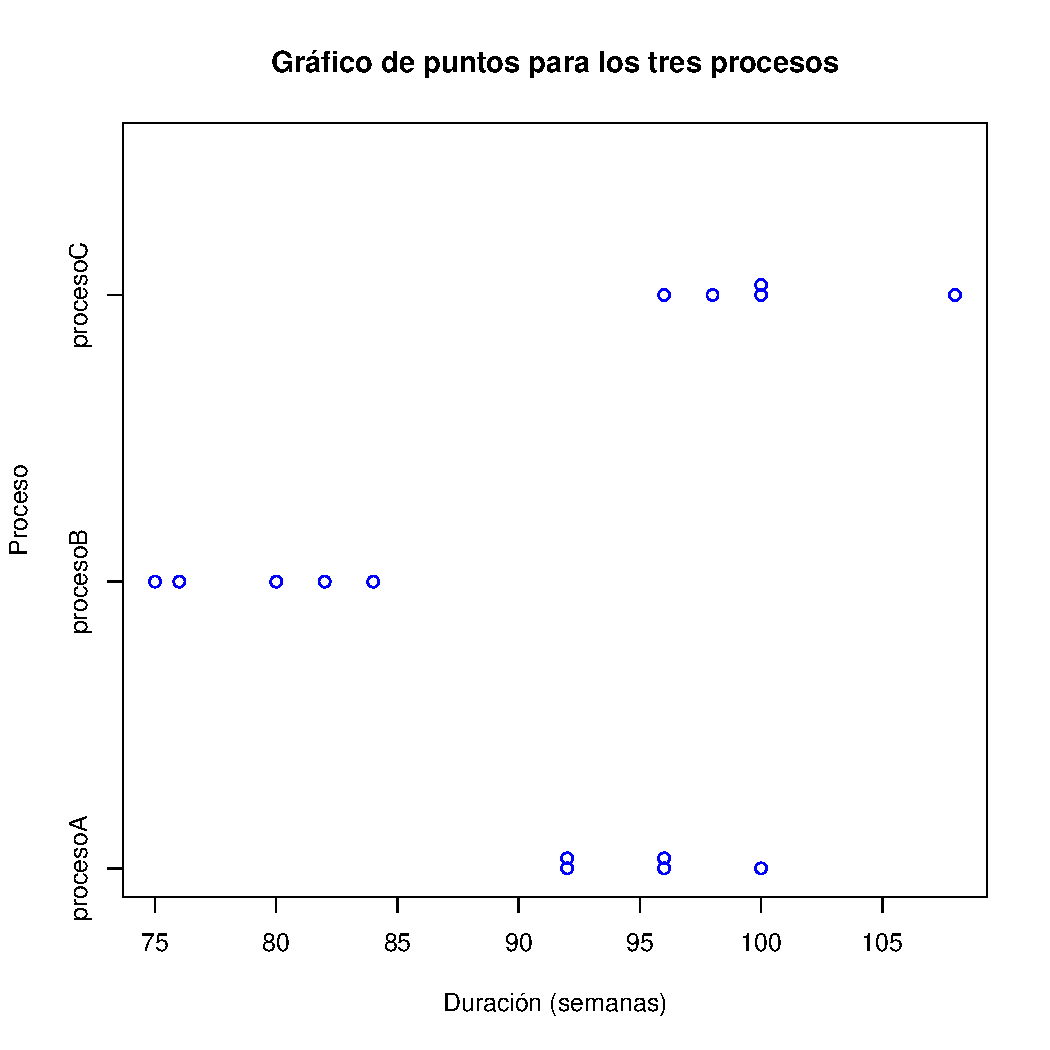
\includegraphics[width=\maxwidth]{figure/unnamed-chunk-8-1} 
\begin{kframe}\begin{alltt}
\hlcom{# Note que con ayuda de este grafico podemos observar si los tres procesos }
\hlcom{# se comportan de manera distinta o parecida en cuanto a duracion en semanas }
\hlcom{# de las baterias. }
\end{alltt}
\end{kframe}
\end{knitrout}

\item  Muestra un resumen estad\'istico para los tres procesos.

\begin{knitrout}
\definecolor{shadecolor}{rgb}{0.969, 0.969, 0.969}\color{fgcolor}\begin{kframe}
\begin{alltt}
\hlkwd{summary}\hlstd{(Baterias)}
\end{alltt}
\begin{verbatim}
##     procesoA        procesoB       procesoC    
##  Min.   : 92.0   Min.   :75.0   Min.   : 96.0  
##  1st Qu.: 92.0   1st Qu.:76.0   1st Qu.: 98.0  
##  Median : 96.0   Median :80.0   Median :100.0  
##  Mean   : 95.2   Mean   :79.4   Mean   :100.4  
##  3rd Qu.: 96.0   3rd Qu.:82.0   3rd Qu.:100.0  
##  Max.   :100.0   Max.   :84.0   Max.   :108.0
\end{verbatim}
\end{kframe}
\end{knitrout}

\item Dibuja un gr\'afico de cajas (box-plot) para los tres procesos.

\begin{knitrout}
\definecolor{shadecolor}{rgb}{0.969, 0.969, 0.969}\color{fgcolor}\begin{kframe}
\begin{alltt}
\hlcom{# Horizontal }

\hlkwd{boxplot}\hlstd{(Baterias,} \hlkwc{width}\hlstd{=}\hlkwa{NULL}\hlstd{,} \hlkwc{varwidth}\hlstd{=}\hlnum{TRUE}\hlstd{,names,} \hlkwc{add}\hlstd{=} \hlnum{FALSE}\hlstd{,} \hlkwc{horizontal}
        \hlstd{=} \hlnum{TRUE}\hlstd{,} \hlkwc{main}\hlstd{=}\hlstr{"Gráfico de caja por proceso"}\hlstd{,} \hlkwc{border}\hlstd{=}\hlkwd{par}\hlstd{(}\hlstr{"fg"}\hlstd{),}
        \hlkwc{col}\hlstd{=}\hlkwd{c}\hlstd{(}\hlstr{"yellow"}\hlstd{,} \hlstr{"cyan"}\hlstd{,} \hlstr{"red"}\hlstd{),} \hlkwc{xlab} \hlstd{=} \hlstr{"Duración (semanas)"}\hlstd{,}
        \hlkwc{ylab}\hlstd{=}\hlstr{"Proceso"}\hlstd{)}
\end{alltt}
\end{kframe}
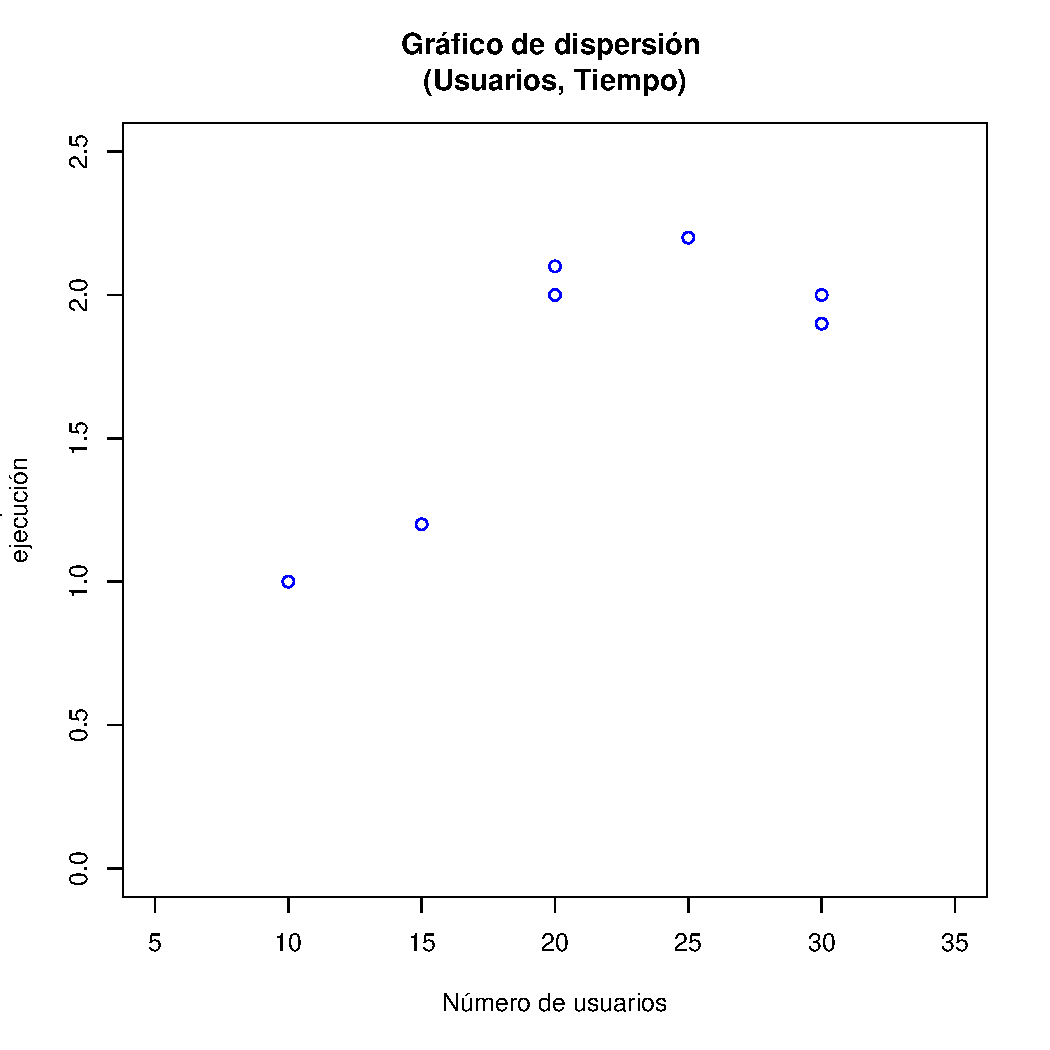
\includegraphics[width=\maxwidth]{figure/unnamed-chunk-10-1} 

\end{knitrout}

\begin{knitrout}
\definecolor{shadecolor}{rgb}{0.969, 0.969, 0.969}\color{fgcolor}\begin{kframe}
\begin{alltt}
\hlcom{# Vertical}

\hlkwd{boxplot}\hlstd{(Baterias,} \hlkwc{width}\hlstd{=}\hlkwa{NULL}\hlstd{,} \hlkwc{varwidth}\hlstd{=}\hlnum{TRUE}\hlstd{,names,} \hlkwc{add}\hlstd{=} \hlnum{FALSE}\hlstd{,} \hlkwc{horizontal}
        \hlstd{=} \hlnum{FALSE}\hlstd{,} \hlkwc{main}\hlstd{=}\hlstr{"Gráfico de caja por proceso"}\hlstd{,} \hlkwc{border}\hlstd{=}\hlkwd{par}\hlstd{(}\hlstr{"fg"}\hlstd{),}
        \hlkwc{col}\hlstd{=}\hlkwd{c}\hlstd{(}\hlstr{"yellow"}\hlstd{,} \hlstr{"cyan"}\hlstd{,} \hlstr{"red"}\hlstd{),} \hlkwc{xlab} \hlstd{=} \hlstr{"Duración (semanas)"}\hlstd{,}
        \hlkwc{ylab}\hlstd{=}\hlstr{"Proceso"}\hlstd{)}
\end{alltt}
\end{kframe}
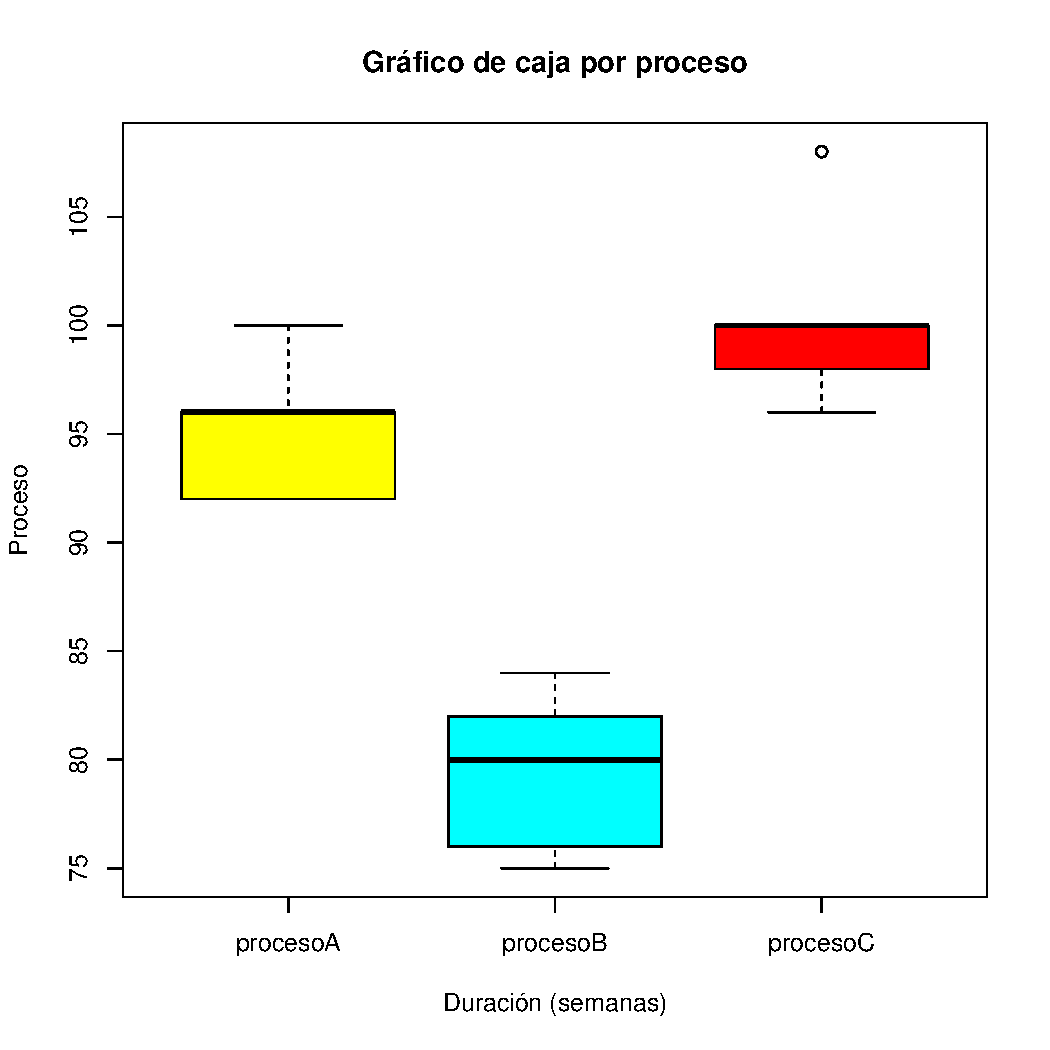
\includegraphics[width=\maxwidth]{figure/unnamed-chunk-11-1} 

\end{knitrout}

\item Presenta la matriz de covarianzas muestral.

\begin{knitrout}
\definecolor{shadecolor}{rgb}{0.969, 0.969, 0.969}\color{fgcolor}\begin{kframe}
\begin{alltt}
\hlkwd{options}\hlstd{(}\hlkwc{digits}\hlstd{=}\hlnum{3}\hlstd{)} \hlcom{# solo imprime 3 lugares decimales }
\hlstd{S} \hlkwb{<-} \hlkwd{var}\hlstd{(Baterias); S}
\end{alltt}
\begin{verbatim}
##          procesoA procesoB procesoC
## procesoA     11.2     -1.6     12.4
## procesoB     -1.6     14.8     -4.7
## procesoC     12.4     -4.7     20.8
\end{verbatim}
\end{kframe}
\end{knitrout}

\item Presenta la desviaci\'on est\'andar de cada proceso. 

\begin{knitrout}
\definecolor{shadecolor}{rgb}{0.969, 0.969, 0.969}\color{fgcolor}\begin{kframe}
\begin{alltt}
 \hlstd{desv} \hlkwb{<-} \hlkwd{sd}\hlstd{(procesoA); desv}
\end{alltt}
\begin{verbatim}
## [1] 3.35
\end{verbatim}
\begin{alltt}
 \hlstd{desv} \hlkwb{<-} \hlkwd{sd}\hlstd{(procesoB); desv}
\end{alltt}
\begin{verbatim}
## [1] 3.85
\end{verbatim}
\begin{alltt}
 \hlstd{desv} \hlkwb{<-} \hlkwd{sd}\hlstd{(procesoC); desv}
\end{alltt}
\begin{verbatim}
## [1] 4.56
\end{verbatim}
\end{kframe}
\end{knitrout}

\item Realiza un an\'alisis de varianza de una v\'ia, para probar la hip\'otesis nula de que el proceso no influye en la duraci\'on de las bater\'ias, es decir, que no hay diferencias entre los tres procesos.

\begin{knitrout}
\definecolor{shadecolor}{rgb}{0.969, 0.969, 0.969}\color{fgcolor}\begin{kframe}
\begin{alltt}
\hlcom{# Concatena los tres vectores dentro de un vector simple, junto con un vector }
\hlcom{# factor indicador de la categoría o tratamiento (A, B, C) que origina cada}
\hlcom{# observacion. El resultado es un data.frame que tiene como componentes los }
\hlcom{# dos vectores anteriores. }
\end{alltt}
\end{kframe}
\end{knitrout}

\begin{knitrout}
\definecolor{shadecolor}{rgb}{0.969, 0.969, 0.969}\color{fgcolor}\begin{kframe}
\begin{alltt}
\hlstd{Baterias} \hlkwb{<-} \hlkwd{stack}\hlstd{(Baterias); Baterias}
\end{alltt}
\begin{verbatim}
##    values      ind
## 1     100 procesoA
## 2      96 procesoA
## 3      92 procesoA
## 4      96 procesoA
## 5      92 procesoA
## 6      76 procesoB
## 7      80 procesoB
## 8      75 procesoB
## 9      84 procesoB
## 10     82 procesoB
## 11    108 procesoC
## 12    100 procesoC
## 13     96 procesoC
## 14     98 procesoC
## 15    100 procesoC
\end{verbatim}
\begin{alltt}
\hlkwd{names}\hlstd{(Baterias)} \hlcom{# Muestra los encabezados de los vectores}
\end{alltt}
\begin{verbatim}
## [1] "values" "ind"
\end{verbatim}
\end{kframe}
\end{knitrout}

\begin{knitrout}
\definecolor{shadecolor}{rgb}{0.969, 0.969, 0.969}\color{fgcolor}\begin{kframe}
\begin{alltt}
\hlcom{# Prueba de igualdad de medias por descomposicion de la varianza en dos }
\hlcom{# fuentes de variacion: la variabilidad que hay entre los grupos (debida a }
\hlcom{# la variable independiente o los tratamientos), y la variabilidad que }
\hlcom{# existe dentro de cada grupo (variabilidad no explicada por los tratamientos). }
\end{alltt}
\end{kframe}
\end{knitrout}

\begin{knitrout}
\definecolor{shadecolor}{rgb}{0.969, 0.969, 0.969}\color{fgcolor}\begin{kframe}
\begin{alltt}
\hlstd{aov.Baterias} \hlkwb{<-} \hlkwd{aov}\hlstd{(values}\hlopt{~}\hlstd{ind,} \hlkwc{data}\hlstd{=Baterias)}

\hlcom{# values~ind relaciona los valores muestrales con los respectivos grupos}

\hlkwd{summary}\hlstd{(aov.Baterias)}
\end{alltt}
\begin{verbatim}
##             Df Sum Sq Mean Sq F value  Pr(>F)    
## ind          2   1196     598    38.3 6.1e-06 ***
## Residuals   12    187      16                    
## ---
## Signif. codes:  0 '***' 0.001 '**' 0.01 '*' 0.05 '.' 0.1 ' ' 1
\end{verbatim}
\begin{alltt}
\hlcom{# Note que es necesario la instruccion anterior para poder visualizar la }
\hlcom{# tabla ANOVA }
\end{alltt}
\end{kframe}
\end{knitrout}

\textbf{Decisi\'on: ya que  a$=$ 0.05 $>$ p-value obtenido, entonces se rechaza Ho}

\begin{knitrout}
\definecolor{shadecolor}{rgb}{0.969, 0.969, 0.969}\color{fgcolor}\begin{kframe}
\begin{alltt}
\hlcom{# Prueba de igualdad de medias en un diseño de una via (o unifactorial) }
\hlcom{# asumiendo  que las varianzas de los grupos son iguales }

\hlkwd{oneway.test}\hlstd{(values}\hlopt{~}\hlstd{ind,} \hlkwc{data}\hlstd{=Baterias,} \hlkwc{var.equal} \hlstd{=} \hlnum{TRUE}\hlstd{)}
\end{alltt}
\begin{verbatim}
## 
## 	One-way analysis of means
## 
## data:  values and ind
## F = 40, num df = 2, denom df = 10, p-value = 6e-06
\end{verbatim}
\end{kframe}
\end{knitrout}

\item Deshace la concatenaci\'on del vector de valores y el vector indicador de categor\'ia. 

\begin{knitrout}
\definecolor{shadecolor}{rgb}{0.969, 0.969, 0.969}\color{fgcolor}\begin{kframe}
\begin{alltt}
\hlstd{Baterias} \hlkwb{=} \hlkwd{unstack}\hlstd{(Baterias);Baterias}
\end{alltt}
\begin{verbatim}
##   procesoA procesoB procesoC
## 1      100       76      108
## 2       96       80      100
## 3       92       75       96
## 4       96       84       98
## 5       92       82      100
\end{verbatim}
\end{kframe}
\end{knitrout}

\item Desconecta la hoja de datos de la segunda ruta o lista de b\'usqueda.

\begin{knitrout}
\definecolor{shadecolor}{rgb}{0.969, 0.969, 0.969}\color{fgcolor}\begin{kframe}
\begin{alltt}
\hlkwd{detach}\hlstd{(Baterias,} \hlkwc{pos}\hlstd{=}\hlnum{2}\hlstd{);} \hlkwd{search}\hlstd{()}
\end{alltt}
\begin{verbatim}
##  [1] ".GlobalEnv"        "package:knitr"     "package:stats"    
##  [4] "package:graphics"  "package:grDevices" "package:utils"    
##  [7] "package:datasets"  "package:methods"   "Autoloads"        
## [10] "package:base"
\end{verbatim}
\end{kframe}
\end{knitrout}

\end{enumerate}

\newpage

\subsection*{EJEMPLO 2}

\subsection*{REALICE UN AN\'ALISIS ESTAD\'ISTICO DE LOS DATOS.}

\begin{enumerate}
\item Activa tu directorio de trabajo.

\begin{knitrout}
\definecolor{shadecolor}{rgb}{0.969, 0.969, 0.969}\color{fgcolor}\begin{kframe}
\begin{alltt}
\hlkwd{getwd}\hlstd{()}
\end{alltt}
\begin{verbatim}
## [1] "C:/Users/User/Documents/PRACTICAS_YOANA_MEDINA/Yoana/PRACTICAS DE R"
\end{verbatim}
\begin{alltt}
\hlkwd{setwd}\hlstd{(}\hlstr{"C:/Curso R2012"}\hlstd{)}
\end{alltt}


{\ttfamily\noindent\bfseries\color{errorcolor}{\#\# Error in setwd("{}C:/Curso R2012"{}): no es posible cambiar el directorio de trabajo}}\end{kframe}
\end{knitrout}

\item Crea un nuevo script y llámale "Script11-DatosBivariados3".

\item Crea dos vectores con los datos. 

\begin{knitrout}
\definecolor{shadecolor}{rgb}{0.969, 0.969, 0.969}\color{fgcolor}\begin{kframe}
\begin{alltt}
\hlstd{Fuma} \hlkwb{=} \hlkwd{c}\hlstd{(}\hlstr{"Si"}\hlstd{,}\hlstr{"No"}\hlstd{,}\hlstr{"No"}\hlstd{,}\hlstr{"Si"}\hlstd{,}\hlstr{"No"}\hlstd{,}\hlstr{"Si"}\hlstd{,}\hlstr{"Si"}\hlstd{,}\hlstr{"Si"}\hlstd{,}\hlstr{"No"}\hlstd{,}\hlstr{"Si"}\hlstd{); Fuma}
\end{alltt}
\begin{verbatim}
##  [1] "Si" "No" "No" "Si" "No" "Si" "Si" "Si" "No" "Si"
\end{verbatim}
\begin{alltt}
\hlstd{Cantidad} \hlkwb{=} \hlkwd{c}\hlstd{(}\hlnum{1}\hlstd{,}\hlnum{2}\hlstd{,}\hlnum{2}\hlstd{,}\hlnum{3}\hlstd{,}\hlnum{3}\hlstd{,}\hlnum{1}\hlstd{,}\hlnum{2}\hlstd{,}\hlnum{1}\hlstd{,}\hlnum{3}\hlstd{,}\hlnum{2}\hlstd{); Cantidad}
\end{alltt}
\begin{verbatim}
##  [1] 1 2 2 3 3 1 2 1 3 2
\end{verbatim}
\end{kframe}
\end{knitrout}

\item  Crea una hoja de datos que tenga comocomponentes o columnas los dos vectores.

\begin{knitrout}
\definecolor{shadecolor}{rgb}{0.969, 0.969, 0.969}\color{fgcolor}\begin{kframe}
\begin{alltt}
\hlstd{Estudia} \hlkwb{<-} \hlkwd{data.frame}\hlstd{(}\hlkwc{Fuma}\hlstd{=Fuma,} \hlkwc{Cantidad}\hlstd{=Cantidad); Estudia}
\end{alltt}
\begin{verbatim}
##    Fuma Cantidad
## 1    Si        1
## 2    No        2
## 3    No        2
## 4    Si        3
## 5    No        3
## 6    Si        1
## 7    Si        2
## 8    Si        1
## 9    No        3
## 10   Si        2
\end{verbatim}
\end{kframe}
\end{knitrout}

\begin{knitrout}
\definecolor{shadecolor}{rgb}{0.969, 0.969, 0.969}\color{fgcolor}\begin{kframe}
\begin{alltt}
\hlcom{# Puedes editar los datos utilizando }

\hlkwd{fix}\hlstd{(Estudia)}
\end{alltt}
\end{kframe}
\end{knitrout}

\item Guarda la hoja de datos en un archivo. 

\begin{knitrout}
\definecolor{shadecolor}{rgb}{0.969, 0.969, 0.969}\color{fgcolor}\begin{kframe}
\begin{alltt}
\hlkwd{write.table}\hlstd{(Estudia,} \hlkwc{file}\hlstd{=}\hlstr{"Estudia.txt"}\hlstd{,} \hlkwc{append}\hlstd{=}\hlnum{FALSE}\hlstd{,} \hlkwc{quote}\hlstd{=}\hlnum{TRUE}\hlstd{,}
            \hlkwc{sep}\hlstd{=}\hlstr{" "}\hlstd{,} \hlkwc{na}\hlstd{=}\hlstr{"NA"}\hlstd{,} \hlkwc{col.names}\hlstd{=}\hlnum{TRUE}\hlstd{)}
\end{alltt}
\end{kframe}
\end{knitrout}

\item Elimina los objetos almacenados enel \'area de trabajo (Workspace). 

\begin{knitrout}
\definecolor{shadecolor}{rgb}{0.969, 0.969, 0.969}\color{fgcolor}\begin{kframe}
\begin{alltt}
\hlkwd{ls}\hlstd{()}
\end{alltt}
\begin{verbatim}
## [1] "aov.Baterias" "Baterias"     "Cantidad"     "desv"        
## [5] "Estudia"      "Fuma"         "S"
\end{verbatim}
\begin{alltt}
\hlkwd{rm}\hlstd{(}\hlkwc{list}\hlstd{=}\hlkwd{ls}\hlstd{(}\hlkwc{all}\hlstd{=}\hlnum{TRUE}\hlstd{))}
\hlkwd{ls}\hlstd{()}
\end{alltt}
\begin{verbatim}
## character(0)
\end{verbatim}
\end{kframe}
\end{knitrout}

\item Recupera desde el archivo la hoja de datos. 

\begin{knitrout}
\definecolor{shadecolor}{rgb}{0.969, 0.969, 0.969}\color{fgcolor}\begin{kframe}
\begin{alltt}
\hlstd{Estudia} \hlkwb{<-} \hlkwd{read.table}\hlstd{(}\hlstr{"Estudia.txt"}\hlstd{,} \hlkwc{header}\hlstd{=}\hlnum{TRUE}\hlstd{)}
\hlstd{Estudia}
\end{alltt}
\begin{verbatim}
##    Fuma Cantidad
## 1    Si        1
## 2    No        2
## 3    No        2
## 4    Si        3
## 5    No        3
## 6    Si        1
## 7    Si        2
## 8    Si        1
## 9    No        3
## 10   Si        2
\end{verbatim}
\end{kframe}
\end{knitrout}

\item Conecta la hoja de datos a la segunda ruta o lista de b\'usqueda,

\begin{knitrout}
\definecolor{shadecolor}{rgb}{0.969, 0.969, 0.969}\color{fgcolor}\begin{kframe}
\begin{alltt}
\hlkwd{attach}\hlstd{(Estudia,} \hlkwc{pos}\hlstd{=}\hlnum{2}\hlstd{)}
\hlkwd{search}\hlstd{()}
\end{alltt}
\begin{verbatim}
##  [1] ".GlobalEnv"        "Estudia"           "package:knitr"    
##  [4] "package:stats"     "package:graphics"  "package:grDevices"
##  [7] "package:utils"     "package:datasets"  "package:methods"  
## [10] "Autoloads"         "package:base"
\end{verbatim}
\end{kframe}
\end{knitrout}

\item Crea una tabla de contigencia o de doble entrada. 

\begin{knitrout}
\definecolor{shadecolor}{rgb}{0.969, 0.969, 0.969}\color{fgcolor}\begin{kframe}
\begin{alltt}
\hlstd{tablaCont} \hlkwb{<-} \hlkwd{table}\hlstd{(Estudia)}
\hlstd{tablaCont}
\end{alltt}
\begin{verbatim}
##     Cantidad
## Fuma 1 2 3
##   No 0 2 2
##   Si 3 2 1
\end{verbatim}
\end{kframe}
\end{knitrout}

\item Calcula las tablas de proporciones o de probabilidades.

\begin{knitrout}
\definecolor{shadecolor}{rgb}{0.969, 0.969, 0.969}\color{fgcolor}\begin{kframe}
\begin{alltt}
\hlkwd{options}\hlstd{(}\hlkwc{digits}\hlstd{=}\hlnum{3}\hlstd{)} \hlcom{# solo imprime 3 lugares decimales}
\end{alltt}
\end{kframe}
\end{knitrout}

\begin{knitrout}
\definecolor{shadecolor}{rgb}{0.969, 0.969, 0.969}\color{fgcolor}\begin{kframe}
\begin{alltt}
\hlcom{# Proporciones basadas en el total de la muestra, la suma de filas y }
\hlcom{# columnas suman 1 }

\hlstd{propTotal} \hlkwb{<-} \hlkwd{prop.table}\hlstd{(tablaCont); propTotal}
\end{alltt}
\begin{verbatim}
##     Cantidad
## Fuma   1   2   3
##   No 0.0 0.2 0.2
##   Si 0.3 0.2 0.1
\end{verbatim}
\end{kframe}
\end{knitrout}

\begin{knitrout}
\definecolor{shadecolor}{rgb}{0.969, 0.969, 0.969}\color{fgcolor}\begin{kframe}
\begin{alltt}
\hlcom{# Proporciones basadas en el total por fila, cada fila suma 1 }

\hlstd{propFila} \hlkwb{<-} \hlkwd{prop.table}\hlstd{(tablaCont,} \hlnum{1}\hlstd{)}
\hlstd{propFila}
\end{alltt}
\begin{verbatim}
##     Cantidad
## Fuma     1     2     3
##   No 0.000 0.500 0.500
##   Si 0.500 0.333 0.167
\end{verbatim}
\end{kframe}
\end{knitrout}

\begin{knitrout}
\definecolor{shadecolor}{rgb}{0.969, 0.969, 0.969}\color{fgcolor}\begin{kframe}
\begin{alltt}
\hlcom{# Proporciones basadas en el total por columna, cada columna suma 1 }

\hlstd{propCol} \hlkwb{<-} \hlkwd{prop.table}\hlstd{(tablaCont,} \hlnum{2}\hlstd{)}
\hlstd{propCol}
\end{alltt}
\begin{verbatim}
##     Cantidad
## Fuma     1     2     3
##   No 0.000 0.500 0.667
##   Si 1.000 0.500 0.333
\end{verbatim}
\end{kframe}
\end{knitrout}

\item Construya los gr\'aficos de barras de la variable bidimensional. 

\begin{knitrout}
\definecolor{shadecolor}{rgb}{0.969, 0.969, 0.969}\color{fgcolor}\begin{kframe}
\begin{alltt}
\hlcom{# Grafico de barras apiladas con la frecuencia de Cantidad como altura}

\hlkwd{barplot}\hlstd{(}\hlkwd{table}\hlstd{(Estudia}\hlopt{$}\hlstd{Cantidad, Estudia}\hlopt{$}\hlstd{Fuma),} \hlkwc{beside} \hlstd{=} \hlnum{FALSE}\hlstd{,}
\hlkwc{horizontal}\hlstd{=}\hlnum{FALSE}\hlstd{,} \hlkwc{main}\hlstd{=}\hlstr{"Gráfico de barras (Fuma, Cantidad de 
horas de estudio)"}\hlstd{,} \hlkwc{legend.text} \hlstd{=T,} \hlkwc{xlab}\hlstd{=}\hlstr{"Fuma"}\hlstd{,} \hlkwc{ylab}\hlstd{=}\hlstr{"Cantidad de 
horas-estudio"}\hlstd{,}\hlkwc{col}\hlstd{=}\hlkwd{c}\hlstd{(}\hlstr{"yellow"}\hlstd{,} \hlstr{"white"}\hlstd{,} \hlstr{"cyan"}\hlstd{))}
\end{alltt}


{\ttfamily\noindent\color{warningcolor}{\#\# Warning in plot.window(xlim, ylim, log = log, ...): "{}horizontal"{} is not a graphical parameter}}

{\ttfamily\noindent\color{warningcolor}{\#\# Warning in axis(if (horiz) 2 else 1, at = at.l, labels = names.arg, lty = axis.lty, : "{}horizontal"{} is not a graphical parameter}}

{\ttfamily\noindent\color{warningcolor}{\#\# Warning in title(main = main, sub = sub, xlab = xlab, ylab = ylab, ...): "{}horizontal"{} is not a graphical parameter}}

{\ttfamily\noindent\color{warningcolor}{\#\# Warning in axis(if (horiz) 1 else 2, cex.axis = cex.axis, ...): "{}horizontal"{} is not a graphical parameter}}\end{kframe}
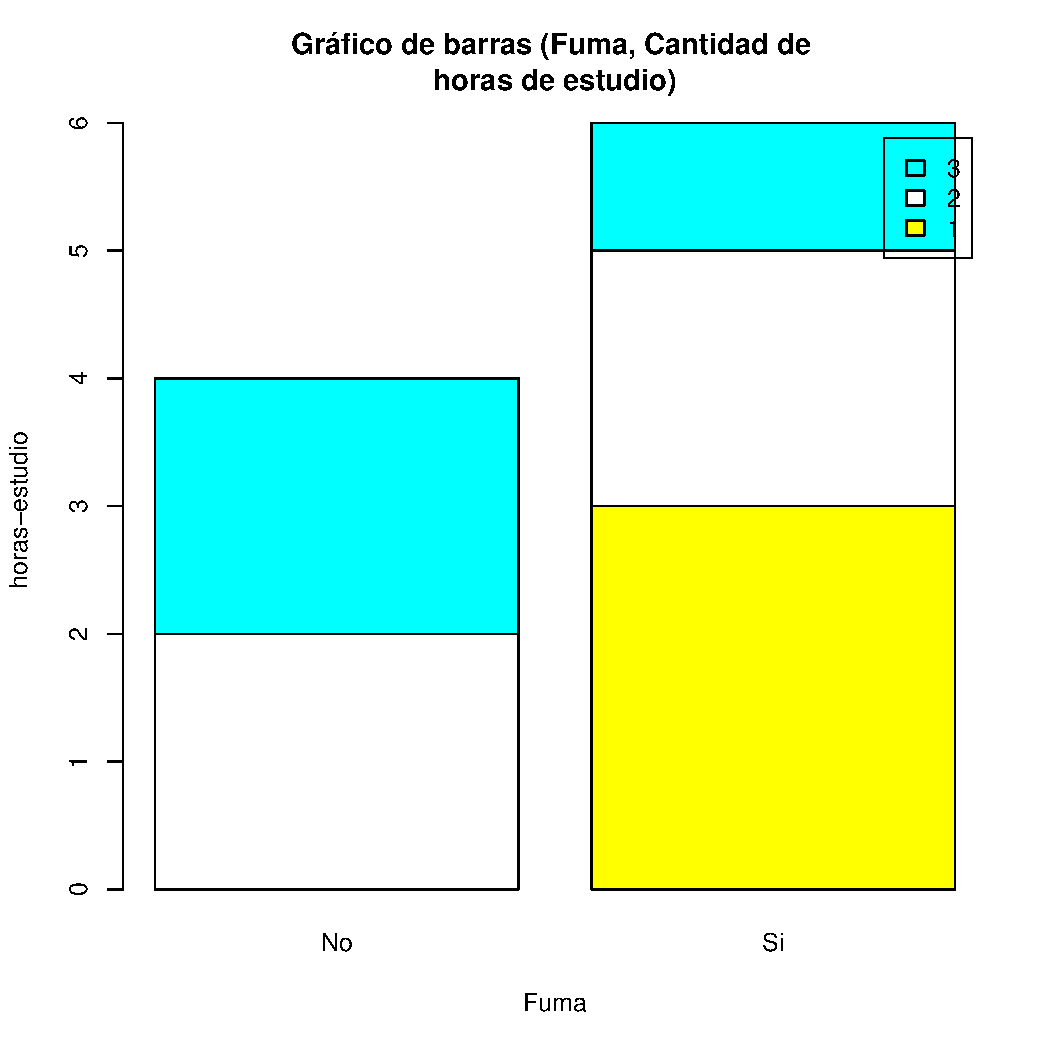
\includegraphics[width=\maxwidth]{figure/unnamed-chunk-34-1} 

\end{knitrout}

\begin{knitrout}
\definecolor{shadecolor}{rgb}{0.969, 0.969, 0.969}\color{fgcolor}\begin{kframe}
\begin{alltt}
\hlcom{# Grafico de barras apiladas con la frecuencia de Fuma como altura}

\hlkwd{barplot}\hlstd{(}\hlkwd{table}\hlstd{(Estudia}\hlopt{$}\hlstd{Fuma, Estudia}\hlopt{$}\hlstd{Cantidad),} \hlkwc{beside} \hlstd{=} \hlnum{FALSE}\hlstd{,}
\hlkwc{horizontal}\hlstd{=}\hlnum{FALSE}\hlstd{,}\hlkwc{main}\hlstd{=}\hlstr{"Gráfico de barras (Cantidad de horas de 
estudio,Fuma)"}\hlstd{,} \hlkwc{legend.text} \hlstd{=T,} \hlkwc{xlab}\hlstd{=}\hlstr{"Cantidad de horas-estudio"}\hlstd{,}
\hlkwc{ylab}\hlstd{=}\hlstr{"Fuma"}\hlstd{,}\hlkwc{col}\hlstd{=}\hlkwd{c}\hlstd{(}\hlstr{"yellow"}\hlstd{,} \hlstr{"white"}\hlstd{,} \hlstr{"cyan"}\hlstd{))}
\end{alltt}


{\ttfamily\noindent\color{warningcolor}{\#\# Warning in plot.window(xlim, ylim, log = log, ...): "{}horizontal"{} is not a graphical parameter}}

{\ttfamily\noindent\color{warningcolor}{\#\# Warning in axis(if (horiz) 2 else 1, at = at.l, labels = names.arg, lty = axis.lty, : "{}horizontal"{} is not a graphical parameter}}

{\ttfamily\noindent\color{warningcolor}{\#\# Warning in title(main = main, sub = sub, xlab = xlab, ylab = ylab, ...): "{}horizontal"{} is not a graphical parameter}}

{\ttfamily\noindent\color{warningcolor}{\#\# Warning in axis(if (horiz) 1 else 2, cex.axis = cex.axis, ...): "{}horizontal"{} is not a graphical parameter}}\end{kframe}
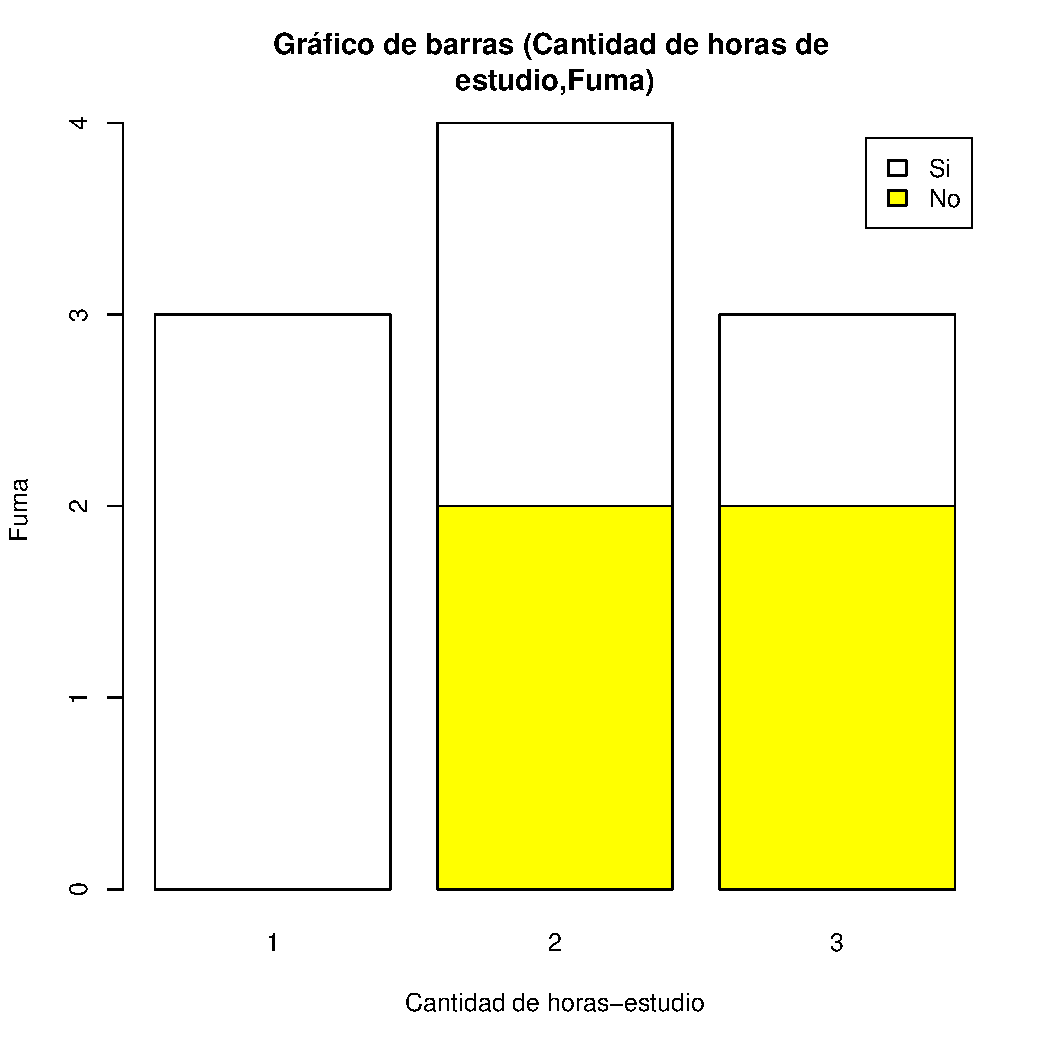
\includegraphics[width=\maxwidth]{figure/unnamed-chunk-35-1} 

\end{knitrout}

\begin{knitrout}
\definecolor{shadecolor}{rgb}{0.969, 0.969, 0.969}\color{fgcolor}\begin{kframe}
\begin{alltt}
\hlcom{# Grafico de barras no apiladas y colocacion de leyenda }

\hlcom{# Crear un factor para los nombres en la leyenda }

\hlstd{Fuma}\hlkwb{=}\hlkwd{factor}\hlstd{(Estudia}\hlopt{$}\hlstd{Fuma); Fuma}
\end{alltt}
\begin{verbatim}
##  [1] Si No No Si No Si Si Si No Si
## Levels: No Si
\end{verbatim}
\end{kframe}
\end{knitrout}

\begin{knitrout}
\definecolor{shadecolor}{rgb}{0.969, 0.969, 0.969}\color{fgcolor}\begin{kframe}
\begin{alltt}
\hlkwd{barplot}\hlstd{(}\hlkwd{table}\hlstd{(Estudia}\hlopt{$}\hlstd{Cantidad, Estudia}\hlopt{$}\hlstd{Fuma),} \hlkwc{main}\hlstd{=}\hlstr{"Gráfico de 
barras (Fuma, Cantidad de horas de estudio)"}\hlstd{,} \hlkwc{xlab}\hlstd{=}\hlstr{"Fuma"}\hlstd{,}
\hlkwc{ylab}\hlstd{=}\hlstr{"Cantidad dehoras-estudio"}\hlstd{,} \hlkwc{beside}\hlstd{=}\hlnum{TRUE}\hlstd{,} \hlkwc{col}\hlstd{=}\hlkwd{c}\hlstd{(}\hlstr{"yellow"}\hlstd{,} \hlstr{"white"}\hlstd{,}
                                                    \hlstr{"cyan"}\hlstd{),}\hlkwc{legend.text}\hlstd{=T)}
\end{alltt}
\end{kframe}
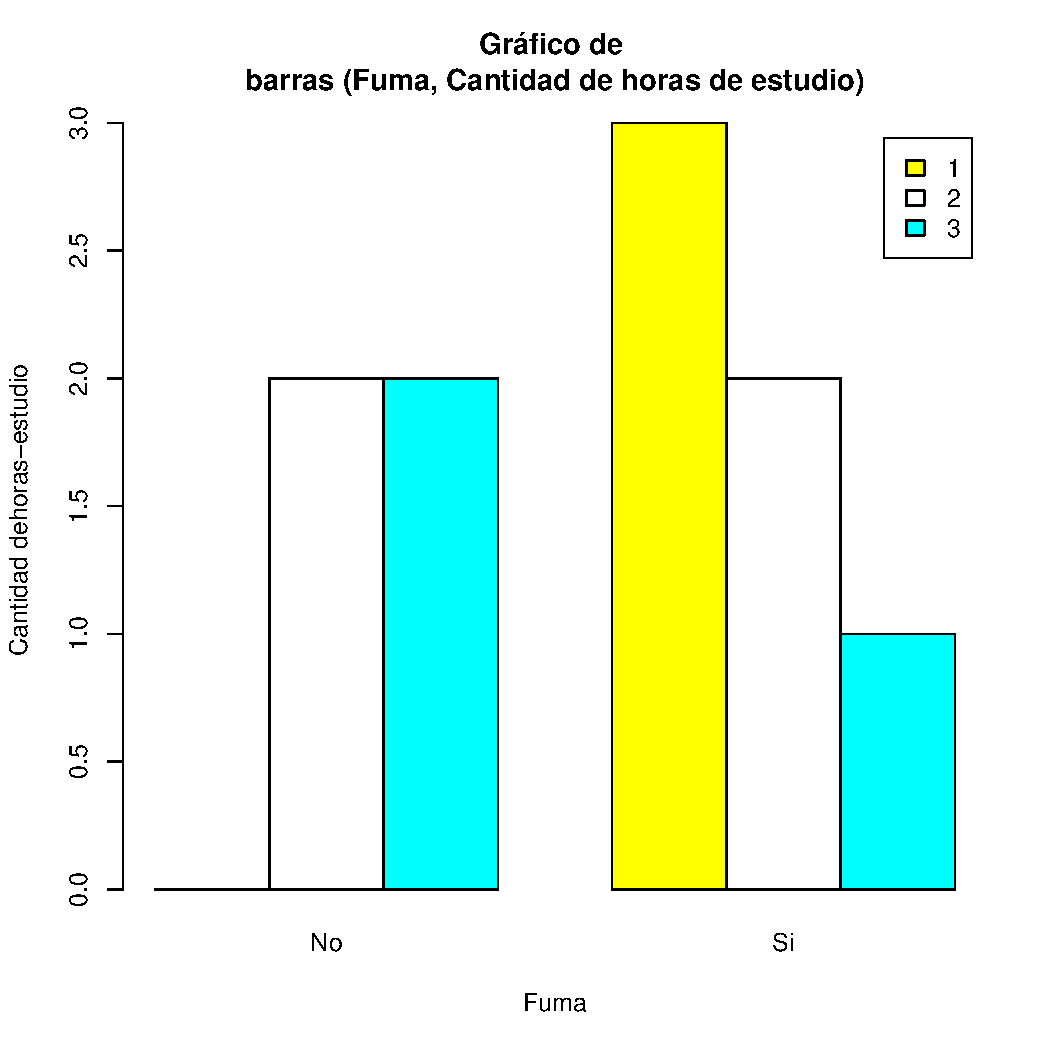
\includegraphics[width=\maxwidth]{figure/unnamed-chunk-37-1} 

\end{knitrout}

\begin{knitrout}
\definecolor{shadecolor}{rgb}{0.969, 0.969, 0.969}\color{fgcolor}\begin{kframe}
\begin{alltt}
\hlkwd{barplot}\hlstd{(}\hlkwd{table}\hlstd{(Estudia}\hlopt{$}\hlstd{Cantidad, Estudia}\hlopt{$}\hlstd{Fuma),} \hlkwc{main}\hlstd{=}\hlstr{"Gráfico de 
barras (Fuma, Cantidad de horas de estudio)"}\hlstd{,} \hlkwc{xlab}\hlstd{=}\hlstr{"Fuma"}\hlstd{,}
\hlkwc{ylab}\hlstd{=}\hlstr{"Cantidad de horas-estudio"}\hlstd{,} \hlkwc{beside}\hlstd{=}\hlnum{TRUE}\hlstd{,} \hlkwc{col}\hlstd{=}\hlkwd{c}\hlstd{(}\hlstr{"yellow"}\hlstd{,}
\hlstr{"white"}\hlstd{,} \hlstr{"cyan"}\hlstd{),}\hlkwc{legend.text}\hlstd{=}\hlkwd{c}\hlstd{(}\hlstr{"menor que 5"}\hlstd{,} \hlstr{"5-10"}\hlstd{,} \hlstr{"mayor que 10"}\hlstd{))}
\end{alltt}
\end{kframe}
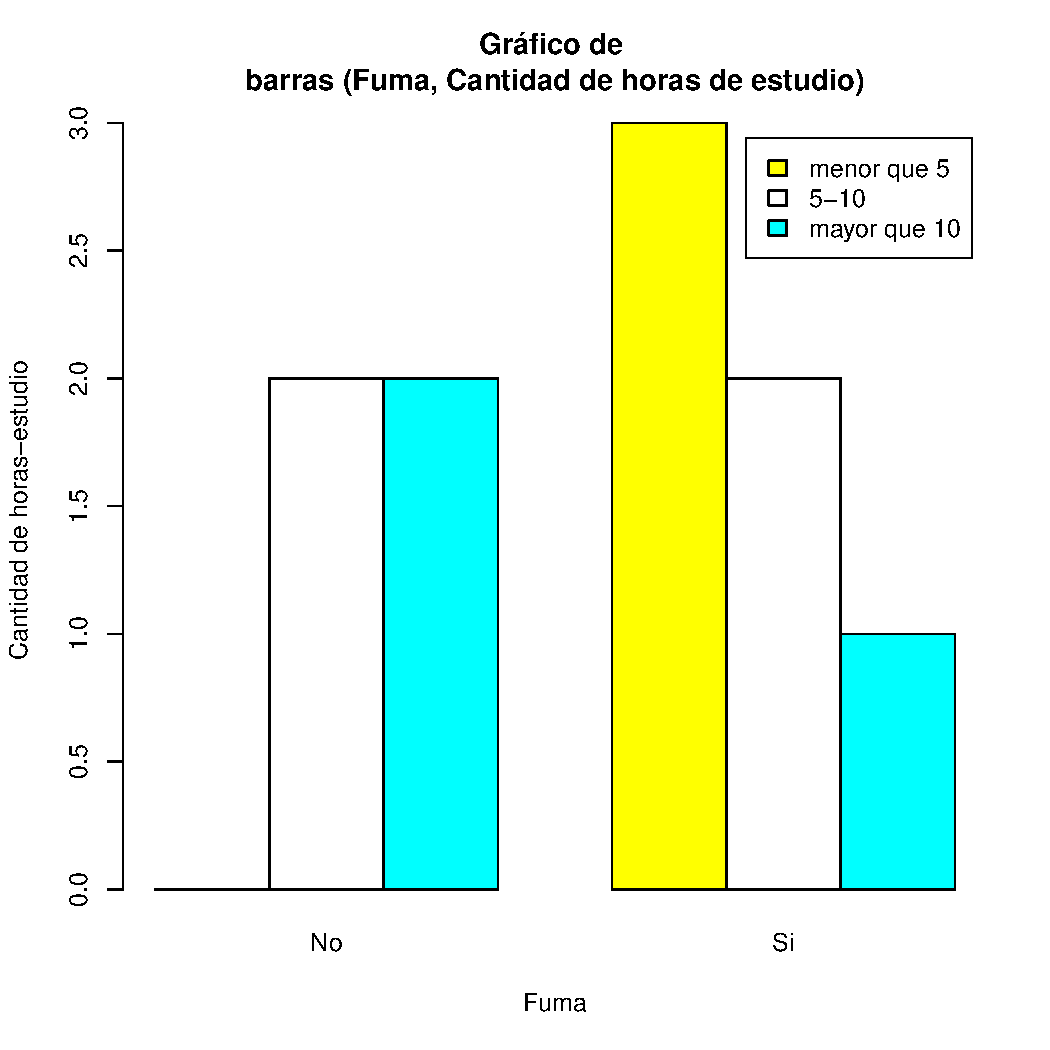
\includegraphics[width=\maxwidth]{figure/unnamed-chunk-38-1} 

\end{knitrout}

\item Realiza la prueba o contraste Chi-cuadrado para las probabilidades dadas 
chisq.test(tablaCont) 

\begin{knitrout}
\definecolor{shadecolor}{rgb}{0.969, 0.969, 0.969}\color{fgcolor}\begin{kframe}
\begin{alltt}
\hlcom{# Si p-value > a aceptar Ho: Las variables son independientes}

\hlcom{# Recuerde que las frecuencias esperadas deben ser mayores a 5 para poder }
\hlcom{# utilizarlas. }
\end{alltt}
\end{kframe}
\end{knitrout}

\begin{knitrout}
\definecolor{shadecolor}{rgb}{0.969, 0.969, 0.969}\color{fgcolor}\begin{kframe}
\begin{alltt}
\hlcom{# Probabilidades esperadas para la prueba Chi-cuadrada}

\hlkwd{chisq.test}\hlstd{(tablaCont)} \hlopt{$}\hlstd{expected}
\end{alltt}


{\ttfamily\noindent\color{warningcolor}{\#\# Warning in chisq.test(tablaCont): Chi-squared approximation may be incorrect}}\begin{verbatim}
##     Cantidad
## Fuma   1   2   3
##   No 1.2 1.6 1.2
##   Si 1.8 2.4 1.8
\end{verbatim}
\end{kframe}
\end{knitrout}








  
  
  
  
  
  
  
  
  
  
  
  
  
  
  
\end{enumerate}













  
  
  
  
  
  
  





\end{document}
